%!Mode:: "TeX:UTF-8"
\section{软件工程开发模型}

\subsection{四大开发模型}
\textbf{瀑布模型(Waterfall Model)}是由W.W.Royce在1970年首次提出的软体开发模型,在瀑布模型中,软件开发被分为需求分析,设计,实现,测试 (确认), 集成,和维护这样的步骤依序进行。Royce提倡重复地使用瀑布模型,以一种迭代的方式。但是,大多数人并不知道这一点,一些人也不相信它能被应用在现实生活中,因为过程很少能够以连续由上而下的方式进行。 经常会需要回到前面的阶段,或改变前一阶段的结果。讽刺的是,在Royce 1970年的那篇文章中他提到:这种模型的目的是作为用来说明这种模式有缺陷,而不适用。事实上,软体开发相关文章中对这个名词的大量引用正是对这个广泛流行的软体开发做法的一种评判。瀑布模型最早强调系统开发应有完整之周期,且必须完整的经历周期之每一开发阶段,并系统化的考量分析与设计的技术、时间与资源之投入等,因此瀑布模型又可以称为‘系统发展生命周期’(System Development Life Cycle, SDLC)。由于该模式强调系统开发过程需有完整的规划、分析、设计、测试及文件等管理与控制,因此能有效的确保系统品质,它已经成为软体业界大多数软件开发的标准。

\textbf{原型模型},即快速应用程式开发 (原名:Rapid Application Development、缩写:RAD)是指一种以最小幅度的规划并迅速地将原形完成的软件发展方法论。采用RAD进行软件开发的规划是和撰写软件本身交错同时进行的。通常能在没有大量预先规划的情况下,让软件更快写完、更容易变更需求。

\textbf{螺旋模型}是一种演化软件开发过程模型,它兼顾了快速原型的迭代的特征以及瀑布模型的系统化与严格监控。螺旋模型最大的特点在于引入了其他模型不具备的风险分析,使软件在无法排除重大风险时有机会停止,以减小损失。同时,在每个迭代阶段构建原型是螺旋模型用以减小风险的途径。螺旋模型更适合大型的昂贵的系统级的软件应用。
\begin{figure}[ht]
	\begin{center}
		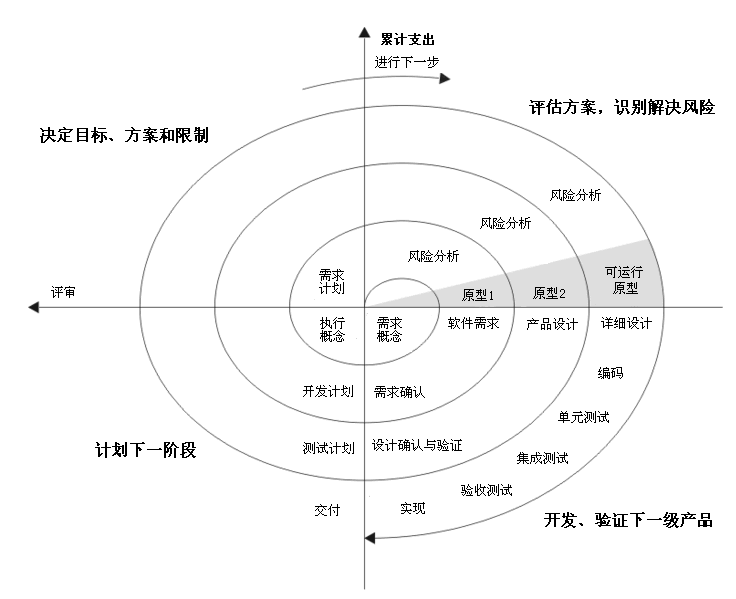
\includegraphics[keepaspectratio,width=0.5\paperwidth]{Pictures/SpiralModelChinese.png}
	\caption{螺旋模型}
	\label{fig:processmemlayout}
	\end{center}
\end{figure}

\textbf{增量模型(incremental build model)}融合了瀑布模型的基本成分(重复应用)和原型实现的迭代特征,该模型采用随着日程时间的进展而交错的线性序列,每一个线性序列产生软件的一个可发布的“增量”。当使用增量模型时,第1个增量往往是核心的产品,即第1个增量实现了基本的需求,但很多补充的特征还没有发布。客户对每一个增量的使用和评估都作为下一个增量发布的新特征和功能,这个过程在每一个增量发布后不断重复,直到产生了最终的完善产品。产品被分解为多个部件,各部件独立设计构建(被称为builds)。每个部件在完成时即时提交给客户,这样就可以利用部分完成的产品,不必等待整个开发期。客户不必一下子接触到一个全新的产品。


\begin{figure}[ht]
	\begin{center}
		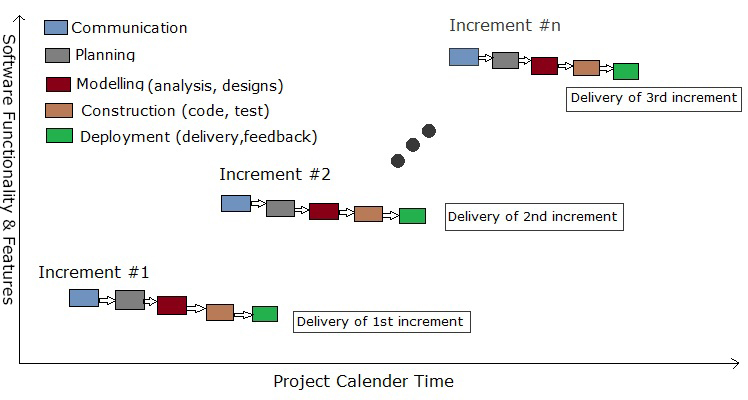
\includegraphics[keepaspectratio,width=0.5\paperwidth]{Pictures/IncrementalModel.jpg}
	\caption{增量模型}
	\label{fig:processmemlayout}
	\end{center}
\end{figure}

\subsection{迭代式开发}
迭代式开发也被称作迭代增量式开发或迭代进化式开发,是一种与传统的瀑布式开发相反的软件开发过程,它弥补了传统开发方式中的一些弱点,具有更高的成功率和生产率。
在迭代式开发方法中,整个开发工作被组织为一系列的短小的、固定长度(如3周)的小项目,被称为一系列的迭代。每一次迭代都包括了需求分析、设计、实现与测试。采用这种方法,开发工作可以在需求被完整地确定之前启动,并在一次迭代中完成系统的一部分功能或业务逻辑的开发工作。再通过客户的反馈来细化需求,并开始新一轮的迭代。

\subsection{敏捷软件开发}
\textbf{敏捷软件开发(Agile software development)},又称敏捷开发,是一种从1990年代开始逐渐引起广泛关注的一些新型软件开发方法,是一种应对快速变化的需求的一种软件开发能力。它们的具体名称、理念、过程、术语都不尽相同,相对于“非敏捷”,更强调程序员团队与业务专家之间的紧密协作、面对面的沟通(认为比书面的文档更有效)、频繁交付新的软件版本、紧凑而自我组织型的团队、能够很好地适应需求变化的代码编写和团队组织方法,也更注重软件开发中人的作用。

敏捷方法有时候被误认为是无计划性和纪律性的方法,实际上更确切的说法是敏捷方法强调适应性而非预见性。
适应性的方法集中在快速适应现实的变化。当项目的需求起了变化,团队应该迅速适应。这个团队可能很难确切描述未来将会如何变化。
相比迭代式开发两者都强调在较短的开发周期提交软件,敏捷方法的周期可能更短,并且更加强调队伍中的高度协作。

通常可以在以下方面衡量敏捷方法的适用性:从产品角度看,敏捷方法适用于需求萌动并且快速改变的情况,如系统有比较高的关键性、可靠性、安全性方面的要求,则可能不完全适合;从组织结构的角度看,组织结构的文化、人员、沟通则决定了敏捷方法是否适用。最重要的因素恐怕是项目的规模。规模增长,面对面的沟通就愈加困难,因此敏捷方法更适用于较小的队伍,40、30、20、10人或者更少。大规模的敏捷软件开发尚处于积极研究的领域。

\subsection{极限编程}
极限编程(Extreme programming,缩写为XP),是一种软件工程方法学,是敏捷软件开发中最富有成效的几种方法学之一。如同其他敏捷方法学,极限编程和传统方法学的本质不同在于它更强调可适应性而不是可预测性。极限编程的支持者认为软件需求的不断变化是很自然的现象,是软件项目开发中不可避免的、也是应该欣然接受的现象;他们相信,和传统的在项目起始阶段定义好所有需求再费尽心思的控制变化的方法相比,有能力在项目周期的任何阶段去适应变化,将是更加现实更加有效的方法。

极限编程为管理人员和开发人员开出了一剂指导日常实践的良方;这个实践意味着接受并鼓励某些特别的有价值的方法。支持者相信,这些在传统的软件工程中看来是“极端的”实践,将会使开发过程比传统方法更加好的响应用户需求,因此更加敏捷,更好的构建出高质量软件。

\subsection{Rational统一过程}
Rational统一过程(RUP)是Rational软件公司(现在Rational公司被IBM并购)创造的软件工程方法。RUP描述了如何有效地利用商业的可靠的方法开发和部署软件,是一种重量级过程(也被称作厚方法学),因此特别适用于大型软件团队开发大型项目。

在软件工程领域,与RUP齐名的软件方法还有:
\begin{itemize}
\item 净室软件工程(重量级)、CMMI(重量级)
\item 极限编程(extreme programming)和其他敏捷软件开发(agile methodology)方法学(轻量级)
\end{itemize}

\subsection{Scrum}

Scrum是一种迭代式增量软件开发过程,通常用于敏捷软件开发。Scrum在英语里是橄榄球运动中争球的意思。
虽然Scrum是为管理软件开发项目而开发的,它同样可以用于运行软件维护团队,或者作为计划管理方法。Scrum之间的合作称为“Scrum of Scrums”。

Scrum是一个包括了一系列实践和预定义角色的过程骨架。Scrum中的主要角色包括:
\begin{enumerate}
\item 'Scrum Master' 是Scrum教练和团队带头人,确保团队合理的运作Scrum,并帮助团队移除实施中的障碍;
\item 产品负责人(Product Owner),确定产品的方向和愿景,定义产品发布的内容、优先级及交付时间,为产品投资报酬率(ROI)负责;
\item 开发团队(Team),一个跨职能的小团队,人数3-9人,团队拥有交付可用软件需要的各种技能。
\end{enumerate}

在每一次冲刺(a sprint or iteration, 一个15到30天的周期,其长度由开发团队决定)当中,开发团队创建可用的(可以随时推出)软件的一个增量。每一个冲刺所要实现的功能来自产品订单(product backlog)。产品订单是按照优先级排列的要完成的工作的概要的需求,哪些订单项会被加入一次冲刺将由冲刺计划会议决定。 在会议中,产品负责人告诉开发团队他需要完成产品订单中的哪些订单项。开发团队决定在下一次冲刺中他们能够承诺完成多少订单项。在冲刺的过程中,没有人能够变更冲刺订单(sprint backlog),这意味着在一个冲刺中需求是被冻结的。

管理Scrum过程有很多实施方法,从即时贴、白板,一直到软件包。Scrum最大的好处之一是它非常容易学习,而且启动Scrum应用并不需要太多的投入。
Scrum会议一共包含以下四种: 1) Sprint计划会议; 2) 每日站立会议; 3) 评审会议; 4) 回顾会议。
在冲刺中,每一天都会举行项目状况会议,被称为“scrum”或“每日站立会议”。
每一个冲刺完成后,都会举行一次冲刺回顾会议,在会议上所有团队成员都要反思这个冲刺。举行冲刺回顾会议是为了进行持续过程改进。会议的时间限制在4小时。
Scrum提倡所有团队成员坐在一起工作,进行口头交流,以及强调项目有关的规范(disciplines),这些有助于创造自我组织的团队。

Scrum的一个关键原则是承认客户可以在项目过程中改变主意,变更他们的需求,而预测式和计划式的方法并不能轻易地解决这种不可预见的需求变化。同样,Scrum采用了经验方法– 承认问题无法完全理解或定义,而是关注于如何使得开发团队快速推出和响应不断出现的需求的能力最大化。










\clearpage